\documentclass[tikz,border=10pt]{standalone}

\begin{document}
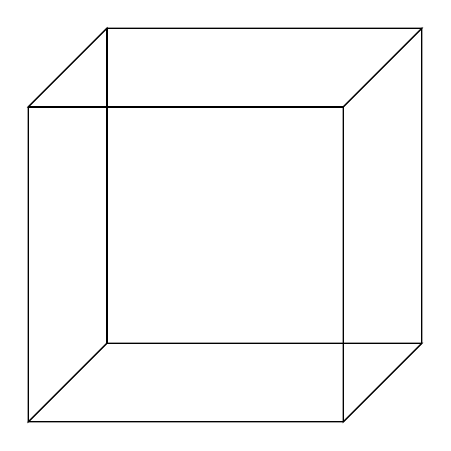
\begin{tikzpicture}[x = {(1cm, 0cm)},
                    y = {(0.25cm, 0.25cm)},
                    z = {(0cm, 1cm)}]

  % draw cube
  \draw (0, 0, 0) -- (0, 4, 0) -- (0, 4, 4) -- (0, 0, 4) -- cycle; % f0
  \draw (4, 0, 0) -- (4, 4, 0) -- (4, 4, 4) -- (4, 0, 4) -- cycle; % f1
  \draw (0, 0, 0) -- (4, 0, 0) -- (4, 0, 4) -- (0, 0, 4) -- cycle; % f2
  \draw (0, 4, 0) -- (4, 4, 0) -- (4, 4, 4) -- (0, 4, 4) -- cycle; % f3
  \draw (0, 0, 0) -- (4, 0, 0) -- (4, 4, 0) -- (0, 4, 0) -- cycle; % f4
  \draw (0, 0, 4) -- (4, 0, 4) -- (4, 4, 4) -- (0, 4, 4) -- cycle; % f5
\end{tikzpicture}
\end{document}
